\documentclass{beamer}

\mode<presentation> {
    \usetheme{Montpellier}

    \usepackage[ddmmyyyy]{datetime}
    \renewcommand{\dateseparator}{.}
    \usepackage{graphicx} % Allows including images
    \usepackage{booktabs} % Allows the use of \toprule, \midrule and \bottomrule in tables
    \usepackage{listings}
    \usepackage{xcolor}
    \setbeamertemplate{caption}{\raggedright\insertcaption\par}
    \addtobeamertemplate{navigation symbols}{}{%
    \usebeamerfont{footline}%
    \usebeamercolor[fg]{footline}%
    \hspace{1em}%
    \insertframenumber/\inserttotalframenumber
}

}

\title[D. Kirchner, Mandelbrotmenge in Hardware]{Entwicklung einer hardwarebeschleunigten Berechnung der Mandelbrotmenge auf einem FPGA} % The short title appears at the bottom of every slide, the full title is only on the title page

\author{Daniel Kirchner}
\institute[HS Coburg]
{
betreut durch: Prof. Oliver Engel\\
Hochschule Coburg
\medskip
}
\date{21.05.2019}

\begin{document}

\frame{\titlepage}

\begin{frame}
    \frametitle{Übersicht}
    \tableofcontents
\end{frame}

\section{Die Mandelbrotmenge}
\begin{frame}
    \frametitle{Die Mandelbrotmenge}
    \begin{itemize}
        \item {nach Benoît Mandelbrot, Begründer des Begriffs "Fraktal"}
        \item lat. \textit{fractus}: gebrochen
        \item selbstähnliche Strukturen in Natur und Mathematik
    \end{itemize}
\end{frame}

\begin{frame}
    \frametitle{Fraktale in der Natur}
    \begin{columns}[c]
        \column{.45\textwidth}
            \begin{figure}
            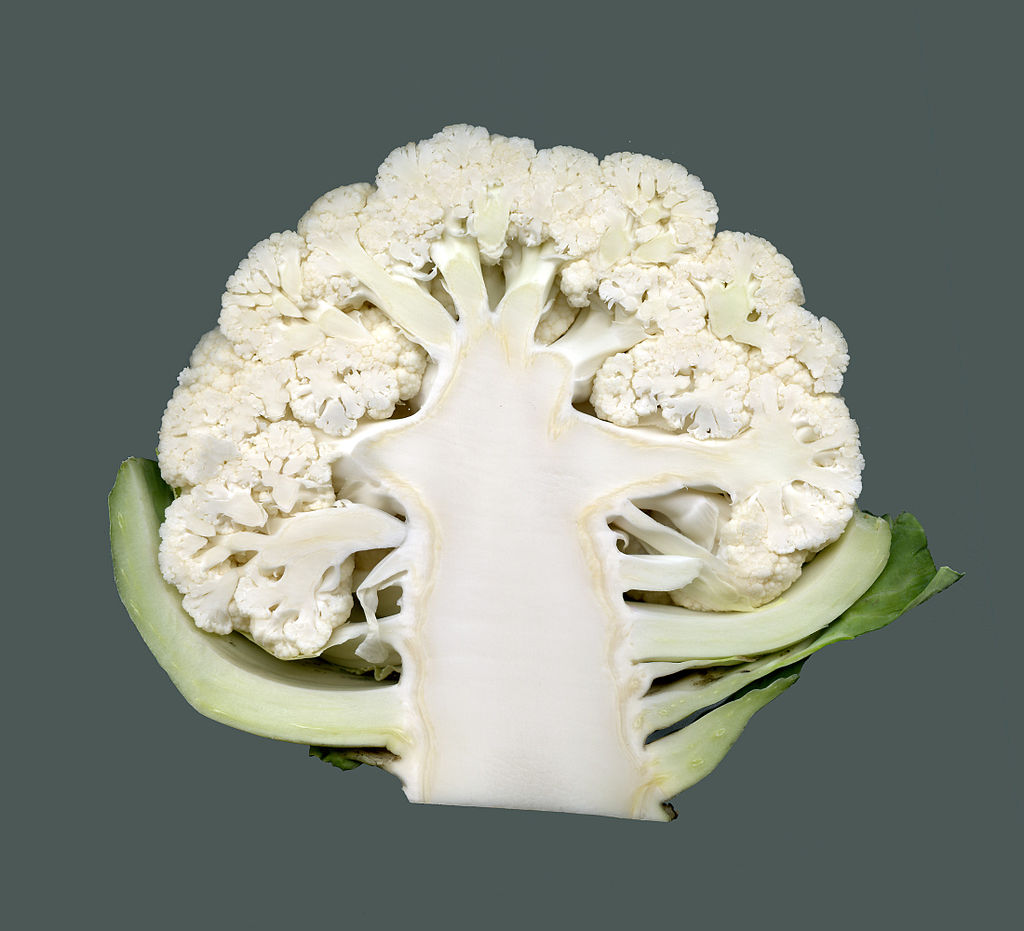
\includegraphics[width=1\linewidth]{img/blumenkohl}
            \caption{Blumenkohl, Rainer Zenz} 
            \end{figure}
        \column{.5\textwidth}
            \begin{figure}
            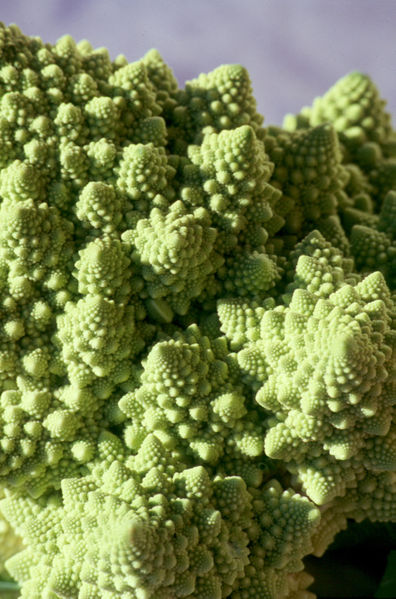
\includegraphics[width=0.7\linewidth]{img/romanesco}
            \caption{Romanesco, Wolfgang Beyer}
            \end{figure}
    \end{columns}
\end{frame}

\begin{frame}
    \centering \textbf{Demonstration:} Fraktaler Baum
\end{frame}

\begin{frame}
    \frametitle{Definition}
    Definiert durch iterative Formel:\\
    \[z_0 = 0\]
    \[z_{n+1} = z_n^2 + c\]
    
    Zur Menge gehören diejenigen $c$, für die die Folge beschränkt ist.
\end{frame}

\begin{frame}
    \centering \textbf{Demonstration:} Konvergenz/Divergenz verschiedener c
\end{frame}

\begin{frame}
    \frametitle{Darstellung}
    \begin{figure}
        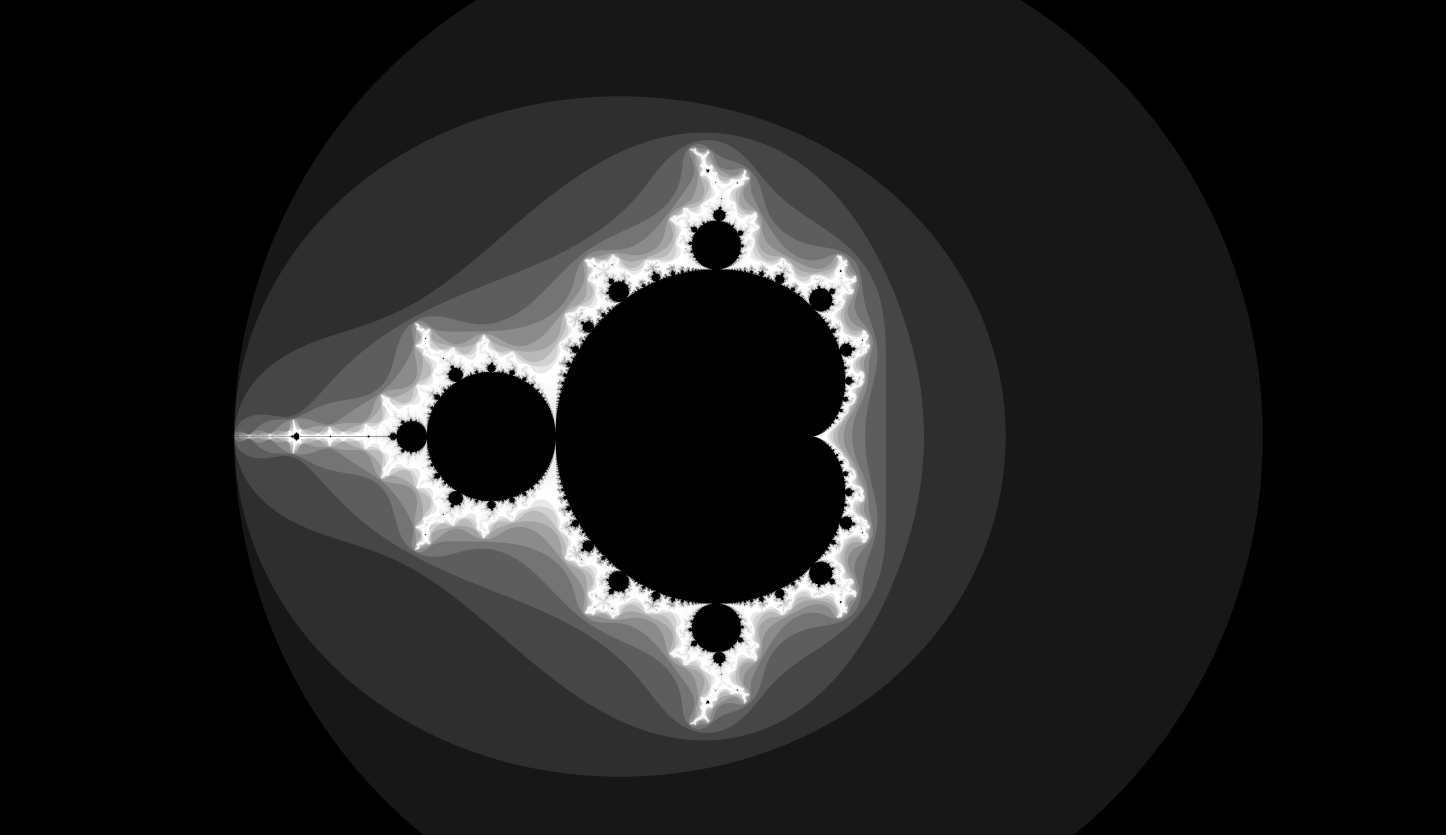
\includegraphics[width=\textwidth]{img/mandelbrot_4.png}
    \end{figure}
\end{frame}

\section{Umsetzung in Hardware}
\begin{frame}
    \frametitle{Umsetzung in Hardware}
    \begin{itemize}
        \item Problem: Visualisierung der Mandelbrotmenge enorm rechenintensiv 
        \item Lösung: Jedoch leicht parallelisierbar, ideal für Hardwareeinsatz
    \end{itemize}
\end{frame}

\begin{frame}
    \frametitle{Gegebene Hardware}
    \begin{columns}[c]
        \column{.45\textwidth}
        Zybo FPGA Trainer Board
        \begin{itemize}
            \item 28.000 Logikzellen
            \item 240 KB Block RAM
            \item 80 DSPs
            \item Dual-Core ARM processor
            \item VGA Output
        \end{itemize}

        \column{.5\textwidth}
        \begin{figure}
            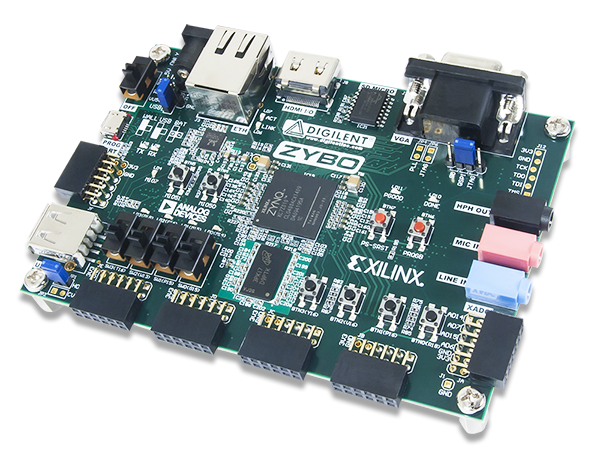
\includegraphics{img/zybo}
            \caption{Zybo Board, Digilent}
        \end{figure}
    \end{columns}
\end{frame}

\begin{frame}
    \frametitle{Komponenten}
    \begin{figure}
        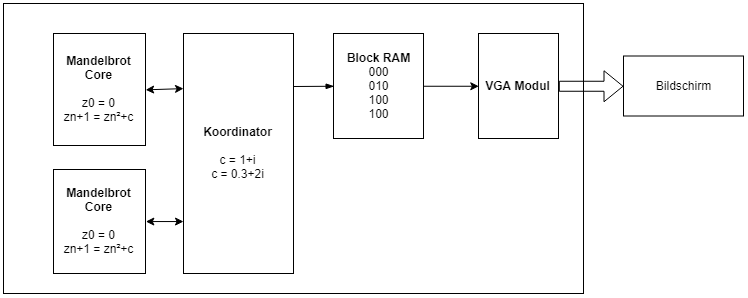
\includegraphics[width=\textwidth]{img/hardware_struktur}
    \end{figure}
\end{frame}

\begin{frame}
    \frametitle{Mandelbrot Core}
    \begin{itemize}
        \item Berechnet für gegebenes c die Anzahl an benötigten Iterationen
        \item Ziel: eine Iteration pro Takt
    \end{itemize}
\end{frame}

\begin{frame}
    \frametitle{Koordinator}
    \begin{itemize}
        \item Übersetzt Pixelkoordinaten in einzelne $c$ Werte
        \item Koordiniert die Inputs der einzelnen Kerne
        \item Schreibt Ergebniswerte (Iterationen) in den BRAM
    \end{itemize}
\end{frame}

\begin{frame}
    \frametitle{VGA Modul / Block RAM}
    \begin{itemize}
        \item Werte im RAM Stellen Iterationsbereich da
        \item 240 KB Block RAM verfügbar
        \item 800x600 Signal mit 3 Bit pro Pixel
        \item 8 Farben pro Pixel
        \item Funktionsweise: Pixel für Pixel auslesen und darstellen
    \end{itemize}
\end{frame}

\begin{frame}
    \frametitle{VGA Modul}
    \begin{figure}
        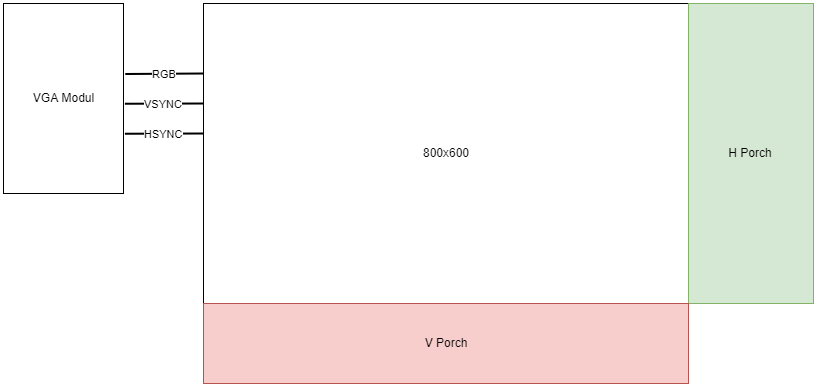
\includegraphics[width=\textwidth]{img/vga.png}
    \end{figure}
\end{frame}

\begin{frame}
    \begin{figure}
        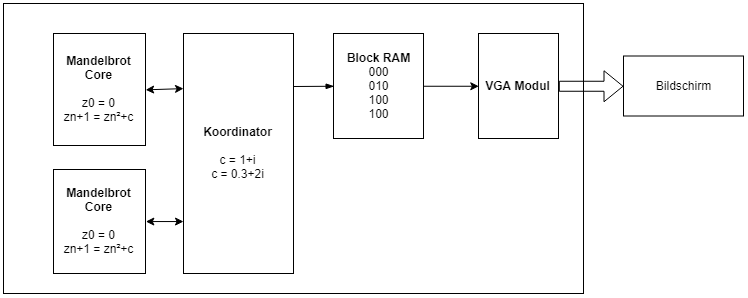
\includegraphics[width=\textwidth]{img/hardware_struktur}
    \end{figure}
\end{frame}

\section{Optimierungen}
\begin{frame}
    \frametitle{Algebraische Optimierungen}
    In jedem Schritt:
    \[z = z^2 + c\]
    und dann Abfrage:
    \[abs(z) <= 2\]
    \color{red}Ziel: \color{black} Minimale Zahl von Multiplikationen
\end{frame}

\begin{frame}
    \[abs(z) <= 2\]
    \[\Leftrightarrow\sqrt{z_r^2 + z_i^2} <= 2\]
    \[\Leftrightarrow z_r^2 + z_i^2 <= 4\]
\end{frame}

\begin{frame}
    \[z = z^2 + c\]
    \[\Leftrightarrow z = z_r^2 - z_i^2 + 2 z_r z_i + c\]
    \[z_r = z_r^2 - z_i^2 + c_r\]
    \[z_i = 2  z_r  z_i + c_i\]
    \[\Leftrightarrow z_i = z_r z_i + z_r z_i + c_i\]
\end{frame}

\begin{frame}
    \[\color{red} z_r^2 \color{black} + \color{blue} z_i^2 \color{black} <= 4\]
    \[z_r = \color{red} z_r^2 \color{black} - \color{blue} z_i^2 \color{black} + c_r\]
    \[z_i = \color{brown} z_r z_i \color{black} + \color{brown} z_r z_i \color{black} + c_i\]
\end{frame}

\begin{frame}
    \frametitle{Designtechnische Optimierungen}
    \begin{itemize}
        \item VGA-Modul und Mandelbrotcores müssen beide auf BRAM zugreifen $\rightarrow$ Dual Port RAM
        \item Mandelbrotmenge ist geschlossen: y zwischen -1.25 und 1.25, x zwischen -2 und 0,5 $\rightarrow$ 
        Punkte außerhalb nicht in Menge
        \item Eigener \textit{signed}-Datenformat
    \end{itemize}
\end{frame}

\begin{frame}
    \frametitle{Zahlenformat}
    \begin{figure}
        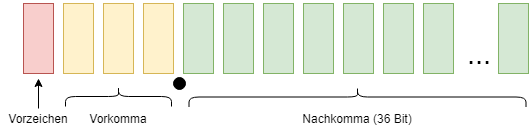
\includegraphics[width=\textwidth]{img/format.png}
    \end{figure}
\end{frame}

{
    \usebackgroundtemplate{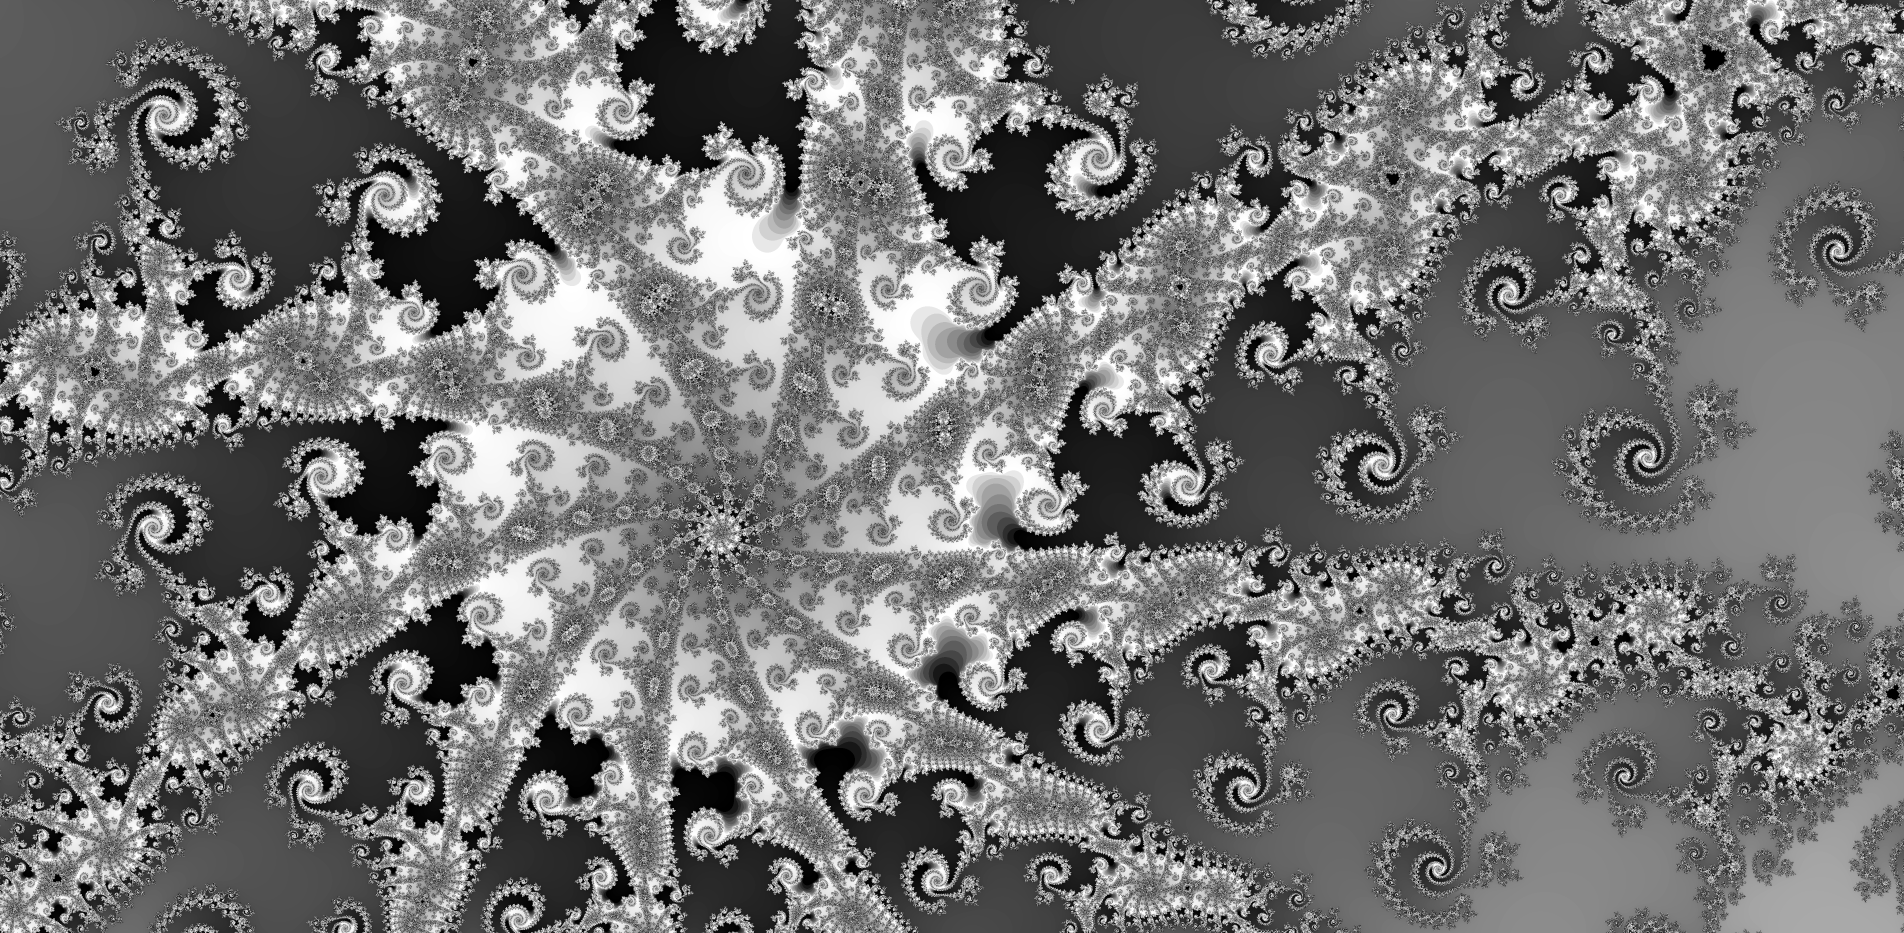
\includegraphics[height=\paperheight,width=\paperwidth]{img/mandelbrot_3.png}}
    \setbeamertemplate{navigation symbols}{}
    \begin{frame}[plain]
    \end{frame}
    }

\end{document} 